% UAIS (Universal Access in the Information Society, Springer) submission version.
% Requires svjour3.cls (download instructions in README.md in this folder).
% Compile with: xelatex main.tex  (twice, for cross-references).

\documentclass[smallextended]{svjour3}

\smartqed  % flush right qed marks, e.g. at end of proof

\usepackage{graphicx}
\usepackage{amsmath,amssymb,amsfonts}
\usepackage{booktabs}
\usepackage{tabularx}
\usepackage{multirow}
\usepackage{float}
\usepackage{url}
\usepackage{hyperref}
\usepackage{fontspec}
\usepackage{kotex}

\journalname{Universal Access in the Information Society}

\begin{document}

\title{KOSHA-Braille: Infrastructure-Grade Accessibility for Korean Chemical Safety Information}
\subtitle{Brief Report}

\titlerunning{KOSHA-Braille}

\author{Yuyong Kim}

\authorrunning{Y. Kim}

\institute{
Yuyong Kim \at
University of Wisconsin--Madison, Madison, WI 53706, USA \\
\email{ykim288@wisc.edu} \\
\textit{ORCID:} 0009-0006-4842-666X
}

\date{}

\maketitle

\begin{abstract}
\textbf{Purpose.} Korean chemical safety information is produced almost entirely as visual regulatory text. This brief report describes KOSHA-Braille, a public Korean Material Safety Data Sheet (MSDS) braille corpus and encoder release intended to provide a baseline accessibility resource for that domain.

\textbf{Methods.} We implement a deterministic Korean braille encoder for the 2017 Korean Braille Standards, apply it to the full KOSHA MSDS database accessed through the Korea Public Data Portal, and cross-validate the output against an independently developed open-source Korean braille converter. The corpus, encoder, decoder, evaluation harness, and reference web deployment are released openly.

\textbf{Results.} The released artifact covers 48{,}966 chemicals over a 769{,}897-row source-section database (401{,}272 sections with substantive Korean text), totaling approximately 119.3~million Korean characters and 232.3~million braille cells. The encoder agrees with the independent reference at 100\% over 442 cross-reference test cases, and the published Korean round-trip golden set is recovered at 45/45.

\textbf{Conclusion.} The contribution is the construction, validation, and public release of a standards-compliant accessibility resource, not an end-user reading-performance claim. Reading-comprehension and field-usability studies with visually impaired readers remain necessary follow-up work.
\keywords{Accessibility infrastructure \and Braille \and Korean braille \and Chemical safety information \and MSDS dataset \and Disability rights}
\end{abstract}

\noindent\textbf{Keywords:} Accessibility infrastructure; Braille; Korean braille; Chemical safety information; MSDS dataset; Disability rights.

\section{Introduction}
\label{sec:introduction}

Material Safety Data Sheets (MSDS), internationally known as Safety Data Sheets, are mandatory technical documents containing hazard classifications, safe handling procedures, emergency measures, and exposure-limit information \cite{kosha_act}. In South Korea these records are produced as visual regulatory text, although information-access obligations under Article~9 of the UN Convention on the Rights of Persons with Disabilities \cite{crpd} and Article~21 of Korea's Anti-Discrimination Against Persons with Disabilities Act \cite{kdpa} provide a clear normative basis for accessible formats. The practical gap is not whether chemical-safety information should be accessible, but whether a reproducible, standards-compliant braille resource exists at the scale of the public MSDS record.

This brief report presents KOSHA-Braille as that resource. The paper's contribution is intentionally narrow: it reports the construction, validation, and public release of a Korean MSDS braille corpus and deterministic encoder. It does not claim to measure end-user reading performance; reading-comprehension and field-usability studies are treated as follow-up work.

The report makes four claims. First, it releases a corpus covering 48{,}966 chemicals from a 769{,}897-row source-section database, with 401{,}272 non-empty Korean sections and approximately 232.3 million braille cells. Second, it implements a deterministic encoder aligned with the 2017 Korean Braille Standards. Third, it validates the encoder against an independent open-source Korean braille converter at 100\% agreement over 442 test cases. Fourth, it releases the dataset, code, verification harness, and reference web service so the resource can be inspected, rebuilt, and reused.

\section{Related Work}
\label{sec:related}

\subsection{Accessibility Infrastructure}

Policy and design literature distinguish \emph{assistive services}, which respond to individual requests, from \emph{accessibility infrastructure}, which pre-installs the conditions for access. Hamraie's history of universal design \cite{hamraie} documents how accessibility provisions originated as targeted disability interventions but were progressively recognized as foundational built-environment features. Blackwell's articulation of the ``curb-cut effect'' \cite{curb_cut} generalizes the pattern: design changes initially intended for an underserved group consistently yield broader benefits, but only after the original intervention has been built ahead of demonstrated demand. Bennett and Keyes \cite{bennett_keyes} further argue that disability-related technical interventions framed in terms of marginal ``fairness'' calculations systematically miss the structural-justice dimension; the appropriate frame is whether the structural conditions for participation exist at all.

The present work positions domain-specific braille corpora for technical and regulatory information as a category of accessibility infrastructure that has been systematically underproduced, particularly outside English. Standard examples---captioning systems, public-library braille collections, audio description, sign-language interpretation of legislative proceedings---are characteristically produced in advance of measured demand and justified by rights frameworks rather than marginal-utility calculations. Within accessibility research specifically, the framings most relevant to the present work are: \emph{ability-based design} and \emph{universal usability}, which treat the absence of access as a property of the artifact rather than the user; the literature on \emph{accessible STEM} and tactile representation, which establishes the precedent that technical content (mathematics, chemistry diagrams) deserves first-class braille and tactile-graphics representation rather than only screen-reader fallbacks; and \emph{disability justice} critiques of marginal-utility framings of accessibility provision. KOSHA-Braille extends this lineage into chemical-safety regulatory documentation, a domain where neither English nor non-English first-class braille infrastructure has previously been reported.

\subsection{Braille Translation Systems and Technical-Material Braille}

Braille translation is most extensively studied for English via liblouis \cite{liblouis}, an open-source translator supporting more than 100 languages. For Korean, liblouis provides Grade~1 and Grade~2 tables based on the 2006 standards; a small number of open-source projects implement the 2017 revisions \cite{hangul_braille_converter,hanbraille}. These tools are character-level translators and do not address domain-level concerns such as consistent handling of regulatory codes, scientific notation within safety text, or large-scale corpus construction.

Beyond character-level translation, prior work on \emph{braille for technical reading} has concentrated on mathematics and STEM education---Nemeth Code and Unified English Braille for mathematical notation, with tooling such as MathML-to-braille pipelines---and on tactile-graphics support for diagrams. Comparatively little work treats large \emph{regulatory} text bodies (statutes, safety documentation, administrative rulings) as a translation target in their own right; existing accessibility provisions for such bodies are typically PDF/HTML accessibility (screen-reader friendliness) rather than first-class braille. The present work positions Korean MSDS as the regulatory analogue of mathematical braille: a domain whose readers need a deterministic, standards-compliant, large-coverage braille representation that they can consume on a refreshable display or embosser without on-the-fly translation.

\subsection{Chemical Safety Information Accessibility}

The Globally Harmonized System (GHS) \cite{ghs} standardizes visual hazard communication but specifies no braille counterpart. The European Union mandates braille on pharmaceutical packaging \cite{eu_braille}, the narrowest precedent for regulated braille in chemistry-adjacent domains; this applies to product names only, not to safety documentation. We are not aware of prior work on braille SDS/MSDS in any language.

\subsection{Korean Braille Standards}

The 2017 Korean Braille Standards \cite{ko_braille_2017} were promulgated by the Ministry of Culture, Sports and Tourism. Korean braille is syllable-structured: each Hangul block decomposes into initial consonant, vowel, and optional final consonant, with each component mapped to a fixed dot pattern. The 2017 revision expanded coverage to six domains including scientific notation and music notation.

\section{System Architecture}
\label{sec:system}

\subsection{Data Pipeline}

The system comprises four stages, illustrated in Fig.~\ref{fig:pipeline}: acquisition, extraction, encoding, and delivery.

\begin{figure}[H]
\centering

\includegraphics[width=0.95\textwidth]{fig_pipeline.png}
\caption{System architecture of KOSHA-Braille. MSDS data is acquired from the KOSHA public API, parsed and cleaned (including GHS pictogram conversion), encoded to Korean braille following the 2017 standards, and served through a web interface.}
\label{fig:pipeline}
\end{figure}

\begin{enumerate}
\item \textbf{Data Acquisition}: KOSHA MSDS data is retrieved via the Korea Public Data Portal REST API \cite{data_go_kr}, providing 16 standardized MSDS sections per chemical in XML format.

\item \textbf{Text Extraction}: XML responses are parsed for Korean text content. GHS pictogram references (e.g., ``GHS06.gif'') are resolved to descriptive Korean text (e.g., ``{급성독성}'') so that braille output conveys semantic hazard information rather than an unreadable filename.

\item \textbf{Braille Encoding}: Korean text is converted to Unicode braille (U+2800--U+28FF) following the 2017 Korean Braille Standards.

\item \textbf{Delivery}: A FastAPI backend serves the encoded content through a REST API; the reference single-page frontend provides search and side-by-side visual/braille viewing; downloads are offered in embosser-format BRF and Unicode \texttt{.txt}.
\end{enumerate}

\subsection{Korean Braille Encoding}

The encoding process is deterministic and lossless. Each Hangul syllable is decomposed using Unicode arithmetic into initial consonant, vowel, and final consonant, each mapping to a fixed dot pattern.

The encoder handles four character types with appropriate braille indicators:

\begin{itemize}
\item \textbf{Hangul}: direct decomposition to braille dot patterns (no indicator needed).
\item \textbf{Numbers}: number indicator (dots 3-4-5-6) followed by digit patterns.
\item \textbf{Latin letters}: Roman letter indicator (dots 3-5-6) followed by letter patterns; uppercase adds capital indicator (dot 6).
\item \textbf{Punctuation}: direct mapping to Korean braille punctuation patterns.
\end{itemize}

Double consonants use a dot-6 prefix cell followed by the base consonant pattern. Compound vowels and compound final consonants use multi-cell sequences.

Tables~\ref{tab:cho}, \ref{tab:jung}, and \ref{tab:jong} show the complete mapping for initial consonants, vowels, and final consonants, respectively. Fig.~\ref{fig:encoding_example} illustrates the full path for two representative MSDS tokens (``메탄올'' = methanol; ``인화성'' = flammable).

\begin{figure}[H]
\centering

\includegraphics[width=0.95\textwidth]{fig_encoding_example.png}
\caption{Worked encoding examples: each Hangul syllable is decomposed into initial/medial/final jamo (blue), then each jamo is emitted as one Korean braille cell. Empty circles denote unused dot positions in a 2$\times$3 braille cell.}
\label{fig:encoding_example}
\end{figure}

\begin{table}[H]
\centering
\caption{Initial Consonant Braille Patterns}
\label{tab:cho}
\begin{tabular}{cccc}
\toprule
Consonant & Dots & Consonant & Dots \\
\midrule
{ㄱ} & 4 & {ㅅ} & 6 \\
{ㄴ} & 1-4 & {ㅇ} & 1-2-4-5 \\
{ㄷ} & 2-4 & {ㅈ} & 4-6 \\
{ㄹ} & 5 & {ㅊ} & 5-6 \\
{ㅁ} & 1-5 & {ㅋ} & 1-2-4 \\
{ㅂ} & 4-5 & {ㅌ} & 1-2-5 \\
& & {ㅍ} & 1-4-5 \\
& & {ㅎ} & 2-4-5 \\
\bottomrule
\end{tabular}
\end{table}

\begin{table}[H]
\centering
\caption{Vowel Braille Patterns}
\label{tab:jung}
\begin{tabular}{cccc}
\toprule
Vowel & Dots & Vowel & Dots \\
\midrule
{ㅏ} & 1-2-6 & {ㅗ} & 1-3-6 \\
{ㅐ} & 1-2-3-5 & {ㅛ} & 3-4-6 \\
{ㅑ} & 3-4-5 & {ㅜ} & 1-3-4 \\
{ㅓ} & 2-3-4 & {ㅠ} & 1-4-6 \\
{ㅔ} & 1-3-4-5 & {ㅡ} & 2-4-6 \\
{ㅕ} & 1-5-6 & {ㅢ} & 2-4-5-6 \\
{ㅖ} & 3-4 & {ㅣ} & 1-3-5 \\
\bottomrule
\end{tabular}
\end{table}

\begin{table}[H]
\centering
\caption{Final Consonant Braille Patterns}
\label{tab:jong}
\begin{tabular}{cccc}
\toprule
Consonant & Dots & Consonant & Dots \\
\midrule
{ㄱ} & 1 & {ㅇ} & 2-3-5-6 \\
{ㄴ} & 2-5 & {ㅈ} & 1-3 \\
{ㄷ} & 3-5 & {ㅊ} & 2-3 \\
{ㄹ} & 2 & {ㅋ} & 2-3-5 \\
{ㅁ} & 2-6 & {ㅌ} & 2-3-6 \\
{ㅂ} & 1-2 & {ㅍ} & 2-5-6 \\
{ㅅ} & 3 & {ㅎ} & 3-5-6 \\
\bottomrule
\end{tabular}
\end{table}

\section{Dataset Description}
\label{sec:dataset}

\subsection{Source Data}

The KOSHA-Braille dataset is derived from the Korea Occupational Safety and Health Agency (KOSHA) Material Safety Data Sheet database, accessed through the Korea Public Data Portal API \cite{data_go_kr} under an authorized operational account with a daily limit of 100,000 calls per endpoint.

\subsection{Dataset Statistics}

Table~\ref{tab:stats} summarizes the dataset characteristics, recomputed directly over the released JSONL artifact. Fig.~\ref{fig:stats} shows the character distribution and the empirical text-length distribution per chemical, and Fig.~\ref{fig:section_coverage} shows per-section coverage and average length.

\begin{figure}[H]
\centering

\includegraphics[width=0.95\textwidth]{fig_dataset_stats.png}
\caption{Dataset characteristics, recomputed from the released JSONL ($n=48{,}966$ chemicals). (Left) character-type distribution. (Right) histogram of per-chemical total Korean text length. The bimodal shape reflects the mix of chemicals with full 16-section MSDS records and chemicals whose KOSHA records contain only a few substantive sections.}
\label{fig:stats}
\end{figure}

\begin{table}[H]
\centering
\caption{KOSHA-Braille Dataset Statistics}
\label{tab:stats}
\begin{tabular}{lr}
\toprule
Metric & Value \\
\midrule
Total chemicals & 48,966 \\
Source-DB section rows & 769,897 \\
Released non-empty sections & 401,272 \\
Avg.\ non-empty sections per chemical & 8.2 (full schema: 16) \\
Korean text (total) & 119.3 M chars \\
Korean braille (total) & 232.3 M cells \\
Mean braille:text ratio & 1.95 \\
\midrule
\multicolumn{2}{l}{\emph{Per-chemical Korean text length}} \\
\quad Mean & 2{,}436 chars \\
\quad Median & 772 chars \\
\quad Std.\ deviation & 2{,}431 chars \\
\quad Min / Max & 0 / 15{,}641 chars \\
\midrule
\multicolumn{2}{l}{\emph{Character type (of classified chars)}} \\
\quad Korean (Hangul) & 77.2\% \\
\quad Latin            & 18.3\% \\
\quad Digits           & 4.5\% \\
\bottomrule
\end{tabular}
\end{table}

\begin{figure}[H]
\centering

\includegraphics[width=0.95\textwidth]{fig_section_coverage.png}
\caption{Per-section coverage of the released dataset over the 16 MSDS sections defined by KOSHA. (a) number of chemicals with non-empty text for each section; sections 1 (chemical/company identification), 3 (composition), 8 (exposure controls), and 14 (transport) are populated for essentially every chemical, while regulatory and physico-chemical detail sections are populated only where the source KOSHA record carries non-placeholder content. (b) average Korean text length per section, conditional on the section being non-empty.}
\label{fig:section_coverage}
\end{figure}

\subsection{GHS Pictogram Conversion}

Original MSDS data references GHS hazard pictograms as image filenames (e.g., ``GHS06.gif''), which are meaningless in braille. The system resolves these to descriptive Korean text as shown in Table~\ref{tab:ghs}. All 147 unique H/P statement codes occurring in the database (63 H-statements, 84 P-statements) are resolved and encoded.

\begin{table}[H]
\centering
\caption{GHS Pictogram to Korean Text Conversion}
\label{tab:ghs}
\begin{tabular}{lll}
\toprule
Code & English & Korean \\
\midrule
GHS01 & Explosive & {폭발성} \\
GHS02 & Flammable & {인화성} \\
GHS03 & Oxidizing & {산화성} \\
GHS04 & Compressed gas & {고압가스} \\
GHS05 & Corrosive & {부식성} \\
GHS06 & Acute toxicity & {급성독성} \\
GHS07 & Irritant & {경고} \\
GHS08 & Health hazard & {건강유해성} \\
GHS09 & Environmental & {수생환경유해성} \\
\bottomrule
\end{tabular}
\end{table}

\subsection{Release}

The full corpus is released as a single JSONL file (943~MB) in HuggingFace-compatible schema, with a dataset card specifying provenance, license, section schema, and intended use. The encoder, decoder, and reference service are released as open-source code.

\section{Validation}
\label{sec:validation}

\subsection{Deterministic Correctness}

Korean braille encoding under the 2017 standards is a deterministic, rule-defined transformation. Each Hangul syllable decomposes unambiguously into initial, medial, and optional final, each mapping to a fixed dot pattern. Correctness therefore reduces to verifying the mapping tables and their application, rather than requiring per-output human-transcriber evaluation---an important property for infrastructure-scale corpora where sample-based human validation cannot reach global coverage.

\subsection{Cross-Reference Validation}

The encoder was validated against an independently developed open-source Korean braille converter \cite{hangul_braille_converter}. Table~\ref{tab:validation} shows the results.

\begin{table}[H]
\centering
\caption{Cross-Reference Validation Results}
\label{tab:validation}
\begin{tabular}{lrr}
\toprule
Test Set & Samples & Agreement \\
\midrule
Basic Hangul syllables & 41 & 100\% \\
Korean golden sentences & 45 & 100\% \\
MSDS chemical names & 356 & 100\% \\
\midrule
\textbf{Total} & \textbf{442} & \textbf{100\%} \\
\bottomrule
\end{tabular}
\end{table}

\subsection{Encoding Properties}

\begin{itemize}
\item \textbf{Deterministic}: identical input always produces identical output.
\item \textbf{Injective}: every distinct Hangul syllable produces a distinct Korean braille string (verified algorithmically by Hangul Unicode decomposition and confirmed across all 442 cross-reference test inputs).
\item \textbf{Standards-compliant}: all dot patterns match the 2017 Korean Braille Standards \cite{ko_braille_2017}.
\end{itemize}

\subsection{Scope of Validation}

This validation establishes correctness of the encoding mapping against a reference implementation and the published standard. Korean round-trip figures, where reported, are interpreted as decoder-path verification under explicit Korean-language dispatch and are not used as evidence against encoder correctness. With the current Korean decoder handling tightened for mixed-script, punctuation, parenthesis, quote, and numeric-span cases, the released golden set now round-trips at 45/45, the persistent stress corpus reports zero failures on 27 mixed-format cases, and repeated random sample spot-checks on the bundled sample DB currently report zero failures. This work does not include a reading-comprehension user study with visually impaired readers, which we identify as essential follow-up work. Grade~2 contracted Korean braille is not implemented; the corpus is Grade~1 throughout.

\section{Reference Deployment}
\label{sec:webservice}

\subsection{Architecture}

The web service is built on FastAPI (Python) with a single-page HTML/JavaScript frontend. SQLite stores pre-fetched MSDS XML; braille conversion is on-demand with typical response times under 500\,ms per chemical.

\subsection{API Endpoints}

\begin{itemize}
\item \texttt{GET /api/stats} -- corpus statistics
\item \texttt{GET /api/chemicals?search=} -- search by Korean name or CAS number
\item \texttt{GET /api/chemicals/\{id\}} -- full MSDS text
\item \texttt{GET /api/chemicals/\{id\}/braille} -- MSDS with Korean braille
\item \texttt{GET /api/chemicals/\{id\}/braille.txt} -- Unicode braille download
\item \texttt{GET /api/chemicals/\{id\}/braille.brf} -- BRF (embosser) download
\item \texttt{POST /api/convert} -- ad-hoc Korean$\rightarrow$braille
\end{itemize}

\subsection{User Interface and Consumption Paths}

The visual side-by-side view (Fig.~\ref{fig:webui}) is a presentation surface for sighted stakeholders (regulators, procurement officers, auditors) who must verify that braille production exists and is consistent with the Korean source. The functionally important outputs for braille readers are the downloadable BRF and Unicode files, which feed directly into: (1) refreshable braille displays over USB or Bluetooth from a local machine or phone; (2) braille embossers for hard-copy output; (3) accessible reading software on desktop and mobile. The deployment is explicitly a reference implementation, not a product; its purpose is to demonstrate that the corpus is consumable end-to-end with existing assistive hardware and software.

\begin{figure}[H]
\centering
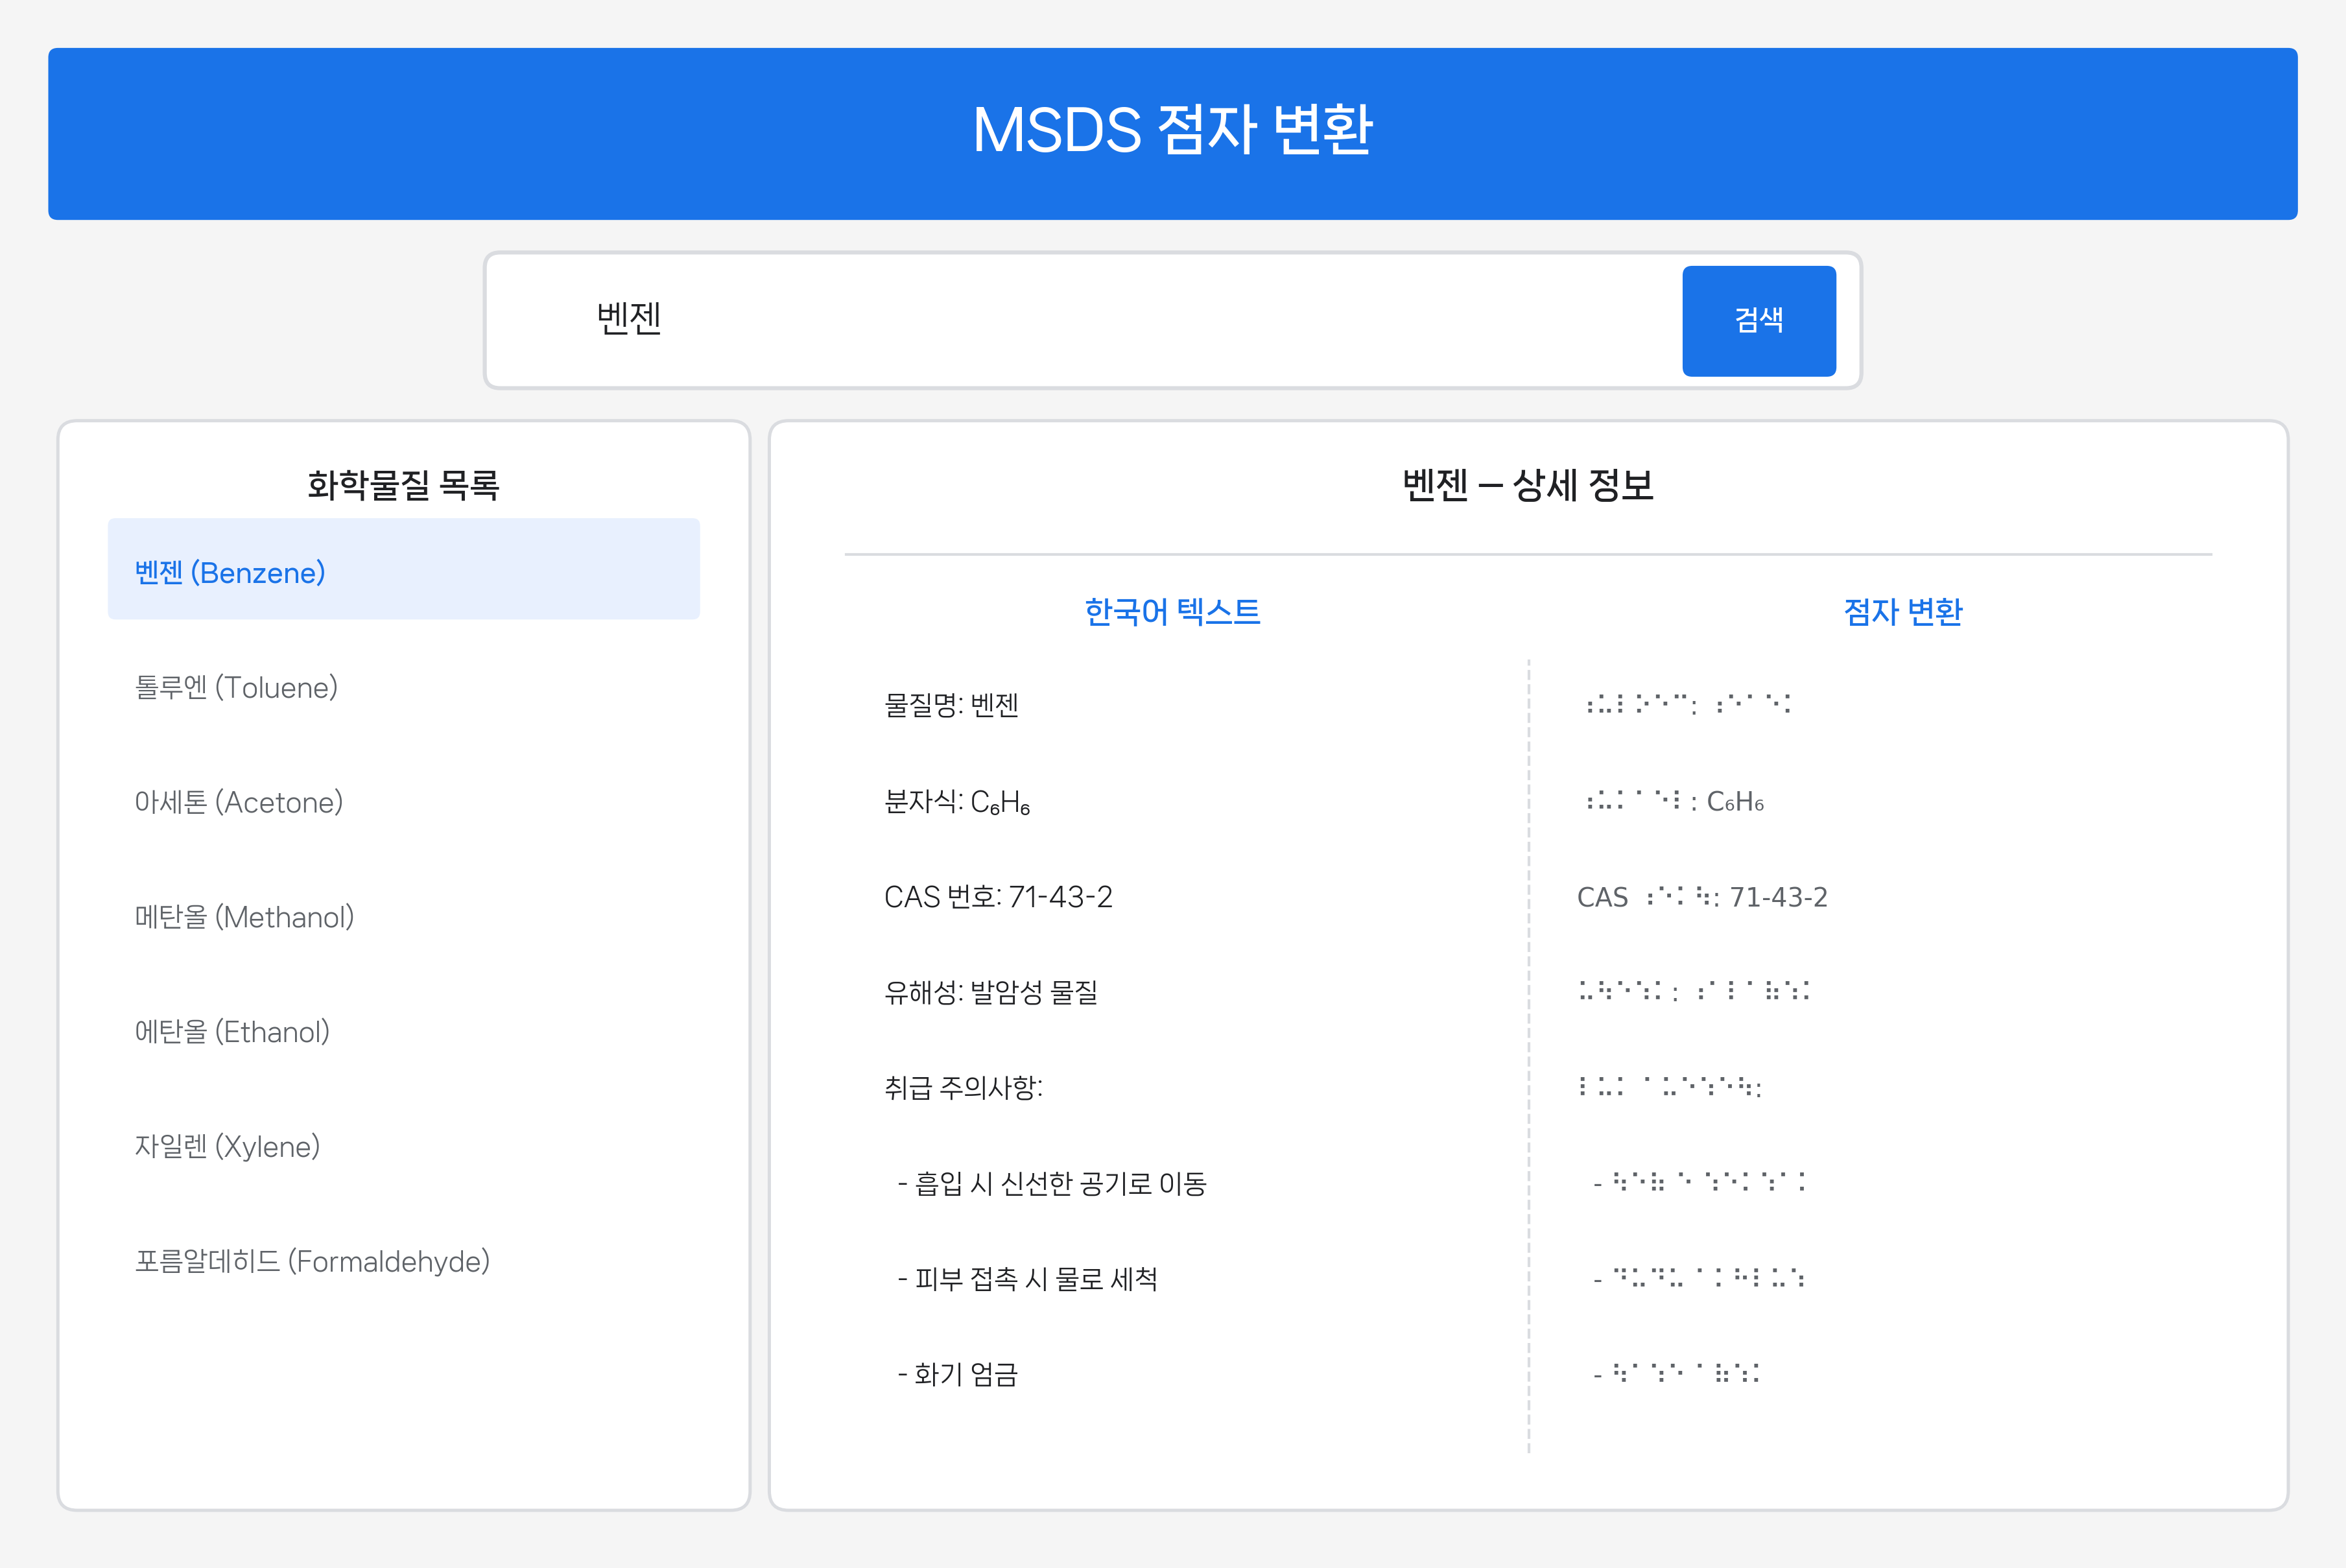
\includegraphics[width=0.95\textwidth]{fig_webui.png}
\caption{Web service user interface showing chemical search (top), result list (left), and side-by-side Korean text and braille display (right).}
\label{fig:webui}
\end{figure}

\section{Extensibility}
\label{sec:extensibility}

The release should not overstate future domains as completed work. We therefore limit the extensibility claim to what the current artifact demonstrates and treat broader uses as future work.

\begin{itemize}
\item \textbf{Validated domain}: the full Korean KOSHA MSDS regime, end-to-end through ingest, GHS text resolution, braille encoding, BRF/Unicode delivery, and reference web service.
\item \textbf{Small extension demonstrations}: Korean food-allergen statements and a 100-record KISCHEM first-aid/occupational-health export exercise the same encoder outside the MSDS corpus, but they are not presented as full second-domain releases.
\item \textbf{Reusable keying}: CAS identifiers provide a bridge to chemical registries without changing the braille encoder, but additional regulatory corpora remain prospective.
\end{itemize}

The reusable pattern is therefore ``structured public-safety source text $\rightarrow$ domain cleaning $\rightarrow$ language-specific braille encoder $\rightarrow$ versioned corpus and downloadable formats.'' Additional regulatory domains are architectural targets for later work, not results claimed by this brief report.

\section{Discussion}
\label{sec:discussion}

KOSHA-Braille is evaluated as an accessibility resource release: coverage of the sighted-reader source, standards compliance, determinism, reproducibility, and public availability. By those criteria the release fills a previously empty Korean chemical-safety braille category.

\paragraph{Validated.}
The encoder implements the 2017 Korean Braille Standards deterministically, agrees with an independent converter at 100\% over 442 cross-reference test cases, and covers every chemical present in the KOSHA MSDS database at release time. The released decoder path also round-trips the 45-sentence Korean golden set at 45/45 and reports zero failures on the persistent 27-case decoder stress corpus.

\paragraph{Not yet validated.}
This report does not measure reading comprehension by visually impaired readers, subjective usability on refreshable displays or embossers, or whether GHS pictogram-to-text resolution is sufficient for hazard recognition. Those are reader-interaction studies, and they require a separate, adequately powered user evaluation built on top of the present resource.

\subsection{Known Limitations}

\begin{enumerate}
\item \textbf{No reading-comprehension user study}: the present release is an infrastructure baseline, not a user-performance study.
\item \textbf{Grade~1 only}: Korean Grade~2 contractions would shorten documents but introduce context-dependent abbreviation decisions incompatible with strict determinism at this stage.
\item \textbf{Decoder ambiguity at the choseong/jongseong boundary}: inherent to Korean braille in the abstract, but the current released Korean decode path now round-trips the published golden set at 45/45; remaining risk is therefore concentrated in unseen real-world edge cases rather than the current benchmark set.
\end{enumerate}

\subsection{Maintenance and Update Model}
\label{sec:maintenance}

Because the upstream KOSHA MSDS database changes over time, the release is versioned rather than treated as a final static authority. The ingest layer can be rerun against the Korea Public Data Portal endpoint, the encoder and verification scripts are open source, and the HuggingFace/GitHub releases allow downstream users to pin a corpus snapshot or rebuild a later one. Single-maintainer risk remains, but the rebuild path is public and reproducible.

\section{Conclusion}
\label{sec:conclusion}

KOSHA-Braille provides a public accessibility resource for Korean chemical safety information: a 48{,}966-chemical, 232.3-million-cell braille corpus produced by a deterministic 2017 Korean Braille Standards encoder and released with code, verification scripts, and a reference deployment. The contribution is the construction, validation, and release of the resource; it is not a claim about end-user reading performance.

The next research step is a separately powered study of reading comprehension and field usability with visually impaired readers, including Grade~2/contracted-braille preferences and tactile or auditory alternatives for hazard pictograms. Until then, the present release serves as the reproducible baseline on which that user-facing work can be built.

\section*{Acknowledgements}

The author thanks the Korea Occupational Safety and Health Agency (KOSHA) for maintaining the Material Safety Data Sheet records used in this work, and the Korea Public Data Portal for providing open API access to those records.

The author also thanks Miss Jayne of Lake Charles, Louisiana, for her enduring warmth and encouragement. The author is deeply grateful to Kyungchul Kim, whose steady presence and thoughtful words have remained a quiet source of guidance.

Finally, the author thanks his parents, Jae-Seob and Soon-Hee, whose support was the kind that needs no words and leaves no debt, and Soul, Yule, June, and Jisun, who are, in the end, the whole point.

\section*{Declarations}

\paragraph{Funding}
This work received no external funding. Compute, infrastructure, and data-portal API access were self-provided.

\paragraph{Competing Interests}
The author declares no competing financial or non-financial interests.

\paragraph{Ethics and Consent}
This work involves no human subjects, no animal subjects, and no personally identifying information. Source data is publicly released regulatory material. Ethics approval, consent to participate, and consent for publication are therefore not applicable.

\paragraph{Author Contributions}
Sole author: conception, design, implementation, validation, analysis, and writing.

\paragraph{Data and Code Availability}
The dataset is released publicly on HuggingFace Datasets as \texttt{Yuyongkim/inconvenience-msds} \cite{hf_dataset}; the encoder, decoder, pipeline, web service, evaluation harness, and the verification scripts used to produce every quantitative claim in this paper are released on GitHub at \texttt{yuyongkim/inconvenience-msds} \cite{github_repo}. The MSDS source data is publicly available through the Korea Public Data Portal \cite{data_go_kr}. Dataset license: CC BY~4.0; code license: MIT.

% Springer Basic style is the journal default (numeric citations).
\bibliographystyle{spbasic}
\bibliography{refs}

\end{document}
